\section{Árvores}

\begin{frame}[fragile]{Características das árvores}

    \begin{itemize}
        \item As {árvores} são estruturas compostas de {nós} e {ramos} (arestas)

        \item Ao contrário das árvores reais, a visualização de árvores em algoritmos é 
            {invertida}, com a {raiz} no topo e as {folhas} na base
        
        \item A {raiz} é um nó que {não tem} pai
        
        \item {Folhas} são nós {que não} tem filhos

        \item Cada nó pode ser alcançado atráves de uma sequência {única}
            de ramos, denominada {caminho}
        

        \item O {nível} de um nó $N$ corresponde ao número de nós do caminho de $N$ até a  raiz 

        \item A {altura} de uma árvore é igual ao {nível máximo} dentre todos os nós da árvore

        \item Uma árvore {vazia} tem altura 0 (zero); uma árvore com {um único} nó tem altura 1

    \end{itemize}

\end{frame}  

\begin{frame}[fragile]{Visualização de uma árvore}

    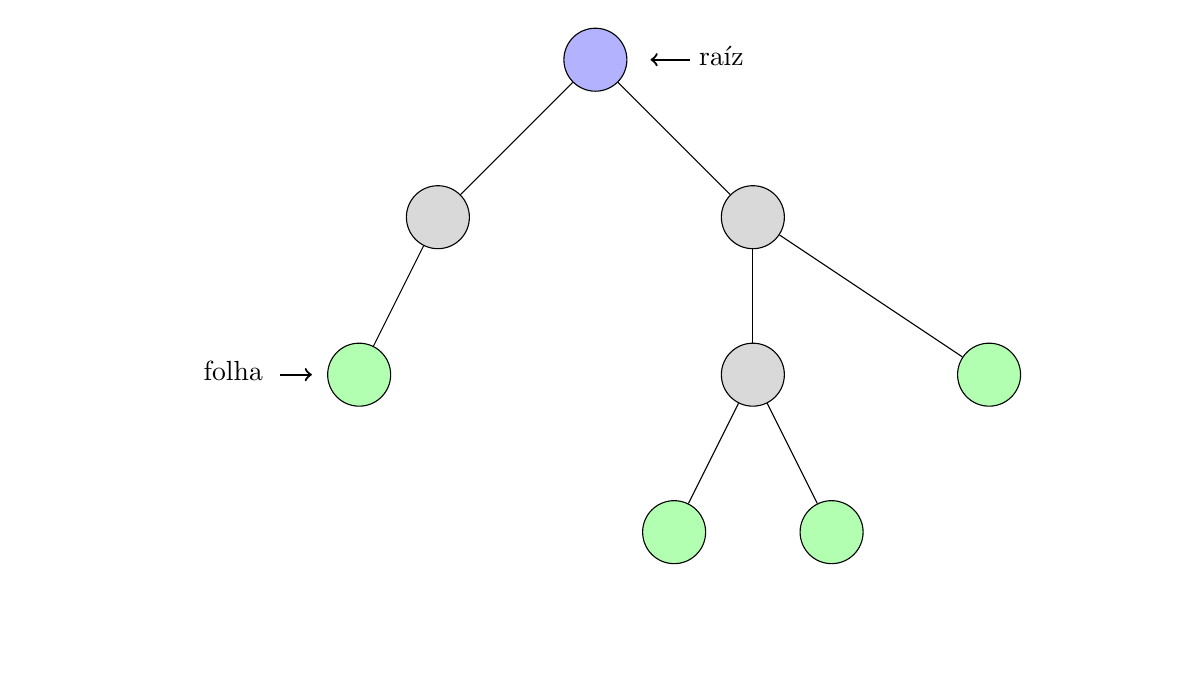
\begin{tikzpicture}
        \node[opacity=0] at (0, 7) { x };
        \node[opacity=0] at (14, 0) { x };
        \node[minimum size=0.8cm, fill=blue!30,circle,draw] (A) at (7, 7.5) { };
        \node[minimum size=0.8cm, fill=gray!30,circle,draw] (B) at (5, 5.5) { };
        \node[minimum size=0.8cm, fill=gray!30,circle,draw] (C) at (9, 5.5) { };
        \node[minimum size=0.8cm, fill=green!30,circle,draw] (D) at (4, 3.5) { };
        \node[minimum size=0.8cm, fill=gray!30,circle,draw] (E) at (9, 3.5) { };
        \node[minimum size=0.8cm, fill=green!30,circle,draw] (F) at (8, 1.5) { };
        \node[minimum size=0.8cm, fill=green!30,circle,draw] (G) at (10, 1.5) { };
        \node[minimum size=0.8cm, fill=green!30,circle,draw] (H) at (12, 3.5) { };

        \draw (A) -- (B);
        \draw (A) -- (C);
        \draw (B) -- (D);
        \draw (C) -- (E);
        \draw (E) -- (F);
        \draw (E) -- (G);
        \draw (C) -- (H);

        \draw[thick,->] (8.2, 7.5) -- (7.7, 7.5);
        \node at (8.6, 7.55) { raíz };

        \draw[thick,->] (3.0, 3.5) -- (3.4, 3.5);
        \node at (2.4, 3.55) { folha };
    \end{tikzpicture}

\end{frame}

\begin{frame}

    \frametitle{Definição formal das árvores}

    As {árvores} são estruturas que podem ser definidas recursivamente da seguinte maneira:
    
    \begin{enumerate}
        \item Uma estrutura {vazia} é uma árvore
        

        \item Se $t_1, t_2, \ldots, t_k$ são árvores disjuntas, então a 
        estrutura cuja {raiz} tem como {filhos} as raizes de 
        $t_1, t_2, \ldots, t_k$ também é uma árvore
        

        \item Apenas estruturas {geradas pelas regras} 1 e 2 são 
        árvores
    \end{enumerate}

\end{frame}
